\documentclass[12pt]{article}

\usepackage[utf8]{inputenc}
\usepackage[margin=1in]{geometry}
\renewcommand{\baselinestretch}{1}
\usepackage{indentfirst}

\usepackage{amsmath, amssymb}

\usepackage{hyperref}
\usepackage{cleveref}
\usepackage{graphicx}
\usepackage{float}
\graphicspath{{./figs/}}

\usepackage{natbib}
\bibliographystyle{aasjournal}

\begin{document}

\begin{center}\begin{LARGE}
\textbf{ASTR 5463 Final Project: ALI Method}
\end{LARGE}\end{center}

\begin{center}
\textbf{Manuel Barrientos, Anthony Burrow, Adam Moss, Sarah Stangl}
\end{center}

\section{Introduction}

Trying to solve the radiative transfer equation in the non-local thermal equilibrium (NLTE) scattering problem is a hard task. In fact, if we want to use a direct approach to solve it, the amount of computer time necessary to find a solution goes over the roof. On the other hand, with the application of an iterative solution technique that uses perturbation operators implicitly in the NLTE solution, we can attack this problem in a more time-efficient way. In particular, in this project, we will use the approach by \citep{OandK1987} which requires the perturbation operator to be an accurate approximation to the diagonal of the lambda matrix.


Explaining lambda iterations,

explaining accelerated lambda interations

parts in the paper

\section{Methods}

subsection
Initial Conditions:

For $i = 2, ..., N - 1$,
\begin{align*}
\alpha_i^-
&=
e_{0, i} +
\frac{e_{2, i} - (\Delta\tau_i + 2\Delta\tau_{i - 1}) e_{1, i}}
     {\Delta\tau_{i - 1} (\Delta\tau_i + \Delta\tau_{i - 1})},
\\ \beta_i^-
&=
\frac{(\Delta\tau_i + \Delta\tau_{i - 1}) e_{1, i} - e_{2, i}}
     {\Delta\tau_{i - 1} \Delta\tau_i}
\\ \gamma_i^-
&=
\frac{e_{2, i} - \Delta\tau_{i - 1} e_{1, i}}
     {\Delta\tau_i (\Delta\tau_i + \Delta\tau_{i - 1})}
\\ \alpha_i^+
&=
\frac{e_{2, i + 1} - \Delta\tau_i e_{1, i + 1}}
     {\Delta\tau_{i - 1} (\Delta\tau_i + \Delta\tau_{i - 1})}
\\ \beta_i^+
&=
\frac{(\Delta\tau_i + \Delta\tau_{i - 1}) e_{1, i + 1} - e_{2, i + 1}}
     {\Delta\tau_{i - 1} \Delta\tau_i}
\\ \gamma_i^+
&=
e_{0, i + 1} +
\frac{e_{2, i + 1} - (\Delta\tau_{i - 1} + 2\Delta\tau_i) e_{1, i + 1}}
     {\Delta\tau_i (\Delta\tau_i + \Delta\tau_{i - 1})},
\end{align*}
where
\begin{align*}
e_{0, i}
&=
1 - e^{-\Delta\tau_{i - 1}},
\\ e_{1, i}
&=
\Delta\tau_{i - 1} - e_{0, i}
\\ e_{2, i}
&=
(\Delta\tau_{i - 1})^2 - 2 e_{1, i}.
\end{align*}

\begin{align*}
\text{i}_{i - 1}^- (\mu, \nu)
&=
\Delta\text{i}_{i - 1}^- (S, \mu, \nu)
\\ &=
\gamma_{i - 1}^-,
\\ \text{i}_{i}^- (\mu, \nu)
&=
\text{i}_{i - 1}^- (\mu, \nu) e^{-\Delta\tau_{i - 1}} +
    \Delta\text{i}_{i}^- (S, \mu, \nu)
\\ &=
\gamma_{i - 1}^- e^{-\Delta\tau_{i - 1}} + \beta_{i}^-,
\\ \text{i}_{i + 1}^- (\mu, \nu)
&=
\text{i}_{i}^- (\mu, \nu) e^{-\Delta\tau_{i - 1}} +
    \Delta\text{i}_{i + 1}^- (S, \mu, \nu)
\\ &=
[\gamma_{i - 1}^- e^{-\Delta\tau_{i - 1}} + \beta_{i}^-] e^{-\Delta\tau_{i}} +
    \alpha_{i + 1}^-,
\end{align*}

\begin{align*}
\text{i}_{i + 1}^+ (\mu, \nu)
&=
\Delta\text{i}_{i + 1}^+ (S, \mu, \nu)
\\ &=
\alpha_{i + 1}^+,
\\ \text{i}_{i}^+ (\mu, \nu)
&=
\text{i}_{i + 1}^+ (\mu, \nu) e^{-\Delta\tau_{i}} +
    \Delta\text{i}_{i}^+ (S, \mu, \nu)
\\ &=
\alpha_{i + 1}^+ e^{-\Delta\tau_{i}} + \beta_{i}^+,
\\ \text{i}_{i - 1}^+ (\mu, \nu)
&=
\text{i}_{i}^+ (\mu, \nu) e^{-\Delta\tau_{i - 1}} +
    \Delta\text{i}_{i - 1}^+ (S, \mu, \nu)
\\ &=
[\alpha_{i + 1}^+ e^{-\Delta\tau_{i}} + \beta_{i}^+] e^{-\Delta\tau_{i - 1}} +
    \gamma_{i - 1}^+.
\end{align*}

\subsection{Ng Acceleration}
Once three iterations have been computed, we can use Ng Acceleration \citep{ng_1974} to compute the next S value and accelerate convergence. Ng Acceleration uses the last 4 S values to compute the next. 

The vectors $\mathbf{S^{n-1}},  \mathbf{S^{n-2}}, \mathbf{S^{n-3}}$ occupy a $\mathbf{2D}$ surface in the linear source function, $\mathbf{S}^{*}$ defined by,

\begin{equation}
    \mathbf{S^{*}} = (1-a-b)\mathbf{S^{n-1}} + a\mathbf{S^{n-2}} + b\mathbf{S^{n-3}}
\end{equation}

for constants $a,b$ such that the next iteration $\mathbf{S^{**}}$,

\begin{equation}
\begin{split}
    \mathbf{S^{**}} &= \epsilon \mathbf{B} +(1-\epsilon)\Lambda \mathbf{S^{*}}\\
    & = (1-a-b)\mathbf{S^{n}} + a\mathbf{S^{n-1}} + b\mathbf{S^{n-2}}
\end{split}
\end{equation}. 

and the magnitude-squared of the difference between the iterations,

\begin{equation}\label{eq:mini}
    | \mathbf{S^{**}} - \mathbf{S^{*}}|^{2} 
\end{equation}

is minimized. The $a,b$ values minimizing Equation \ref{eq:mini} is given by,

\begin{equation}
    a = \frac{C_{1}B_{2}-C_{2}B_{1}}{A_{1}B_{2}-A_{2}B_{1}}
\end{equation}

\begin{equation}
    b = \frac{C_{2}A_{1} - C_{1}A_{2}}{A_{1}B_{2}-A_{2}B_{1}}
\end{equation}

where,

\begin{equation}
\begin{split}
    A_{1} = Q_{1}\cdot Q_{1},\quad B_{1}=Q_{1}\cdot Q_{2},\quad C_{1}=Q_{1}\cdot Q_{3}\\
    A_{2} = Q_{2}\cdot Q_{1},\quad B_{2}=Q_{2}\cdot Q_{2},\quad C_{2}=Q_{2}\cdot Q_{3}
\end{split}
\end{equation}

and 

\begin{equation}
    \begin{split}
        & Q_{1} = \mathbf{S^{n}}-2\mathbf{S^{n-1}}+\mathbf{S^{n-2}}\\
        & Q_{2} = \mathbf{S^{n}}-\mathbf{S^{n-1}}-\mathbf{S^{n-2}}+\mathbf{S^{n-3}}\\
        & Q_{3} = \mathbf{S^{n}}-\mathbf{S^{n-1}}.
    \end{split}
\end{equation}

The new $\mathbf{S^{n+1}}$ is given by,

\begin{equation}
    \mathbf{S^{n+1}} = (1-a-b)\mathbf{S^{n}} + a\mathbf{S^{n-1}} + b\mathbf{S^{n-2}}.
\end{equation}

Before Ng Acceleration can be used again, 3 iterations must pass.


\section{Results and Discussion}

\begin{figure}[ht]
 \centering
 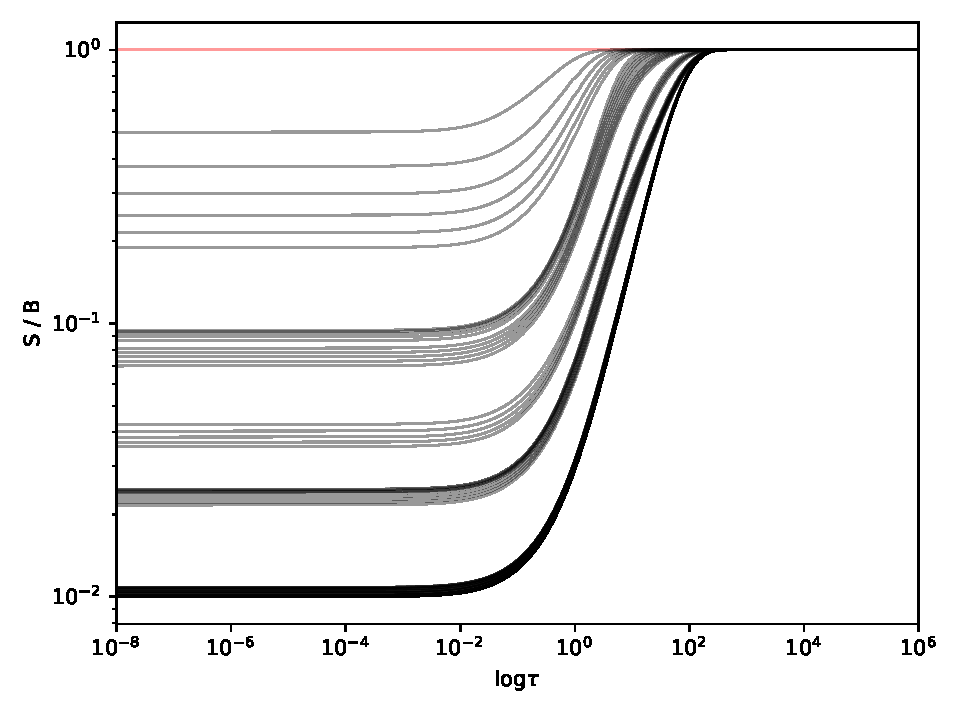
\includegraphics[width=0.75\textwidth]{S_B_convergence.pdf}
 \caption{An example convergence plot with our default parameters using ALI. Each gray line represents a new iteration. At the surface, S/B approaches $\sqrt\epsilon$ while at depth, S/B approaches 1.}
\end{figure}

\begin{figure}[ht]
 \centering
 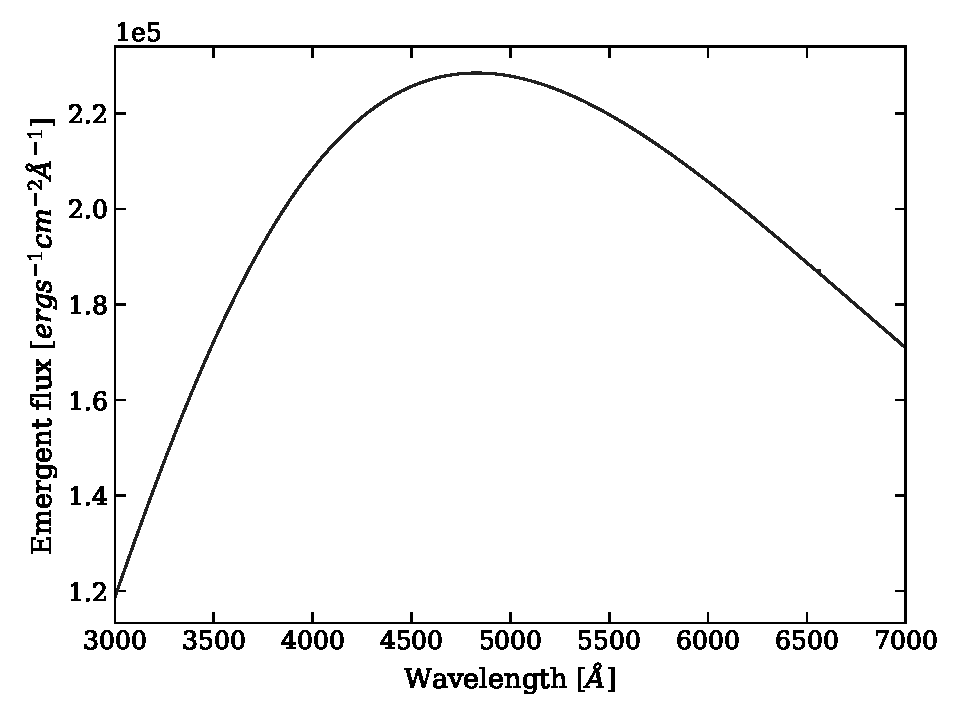
\includegraphics[width=0.75\textwidth]{test_spectrum.pdf}
 \caption{Output spectrum using the default parameters. The line feature at 6564 $\AA$ appears, however the shape is incorrect.}
\end{figure}

\begin{figure}[ht]
 \centering
 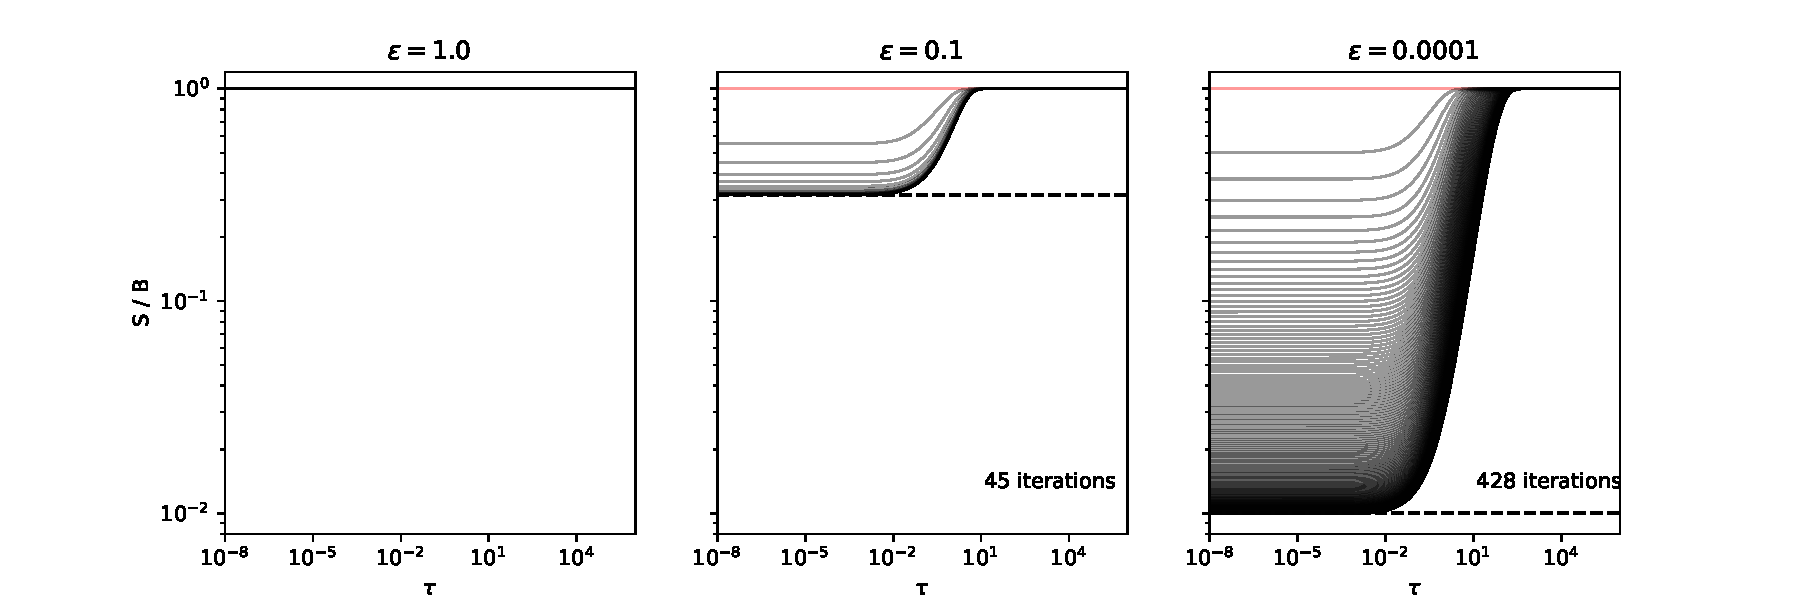
\includegraphics[width=0.99\textwidth]{eps_convergence.pdf}
 \caption{Convergence plots for different values of $\epsilon$. As $\epsilon$ approaches 0, more iterations are needed to achieve convergence at the surface.}
\end{figure}

\begin{figure}[ht]
 \centering
 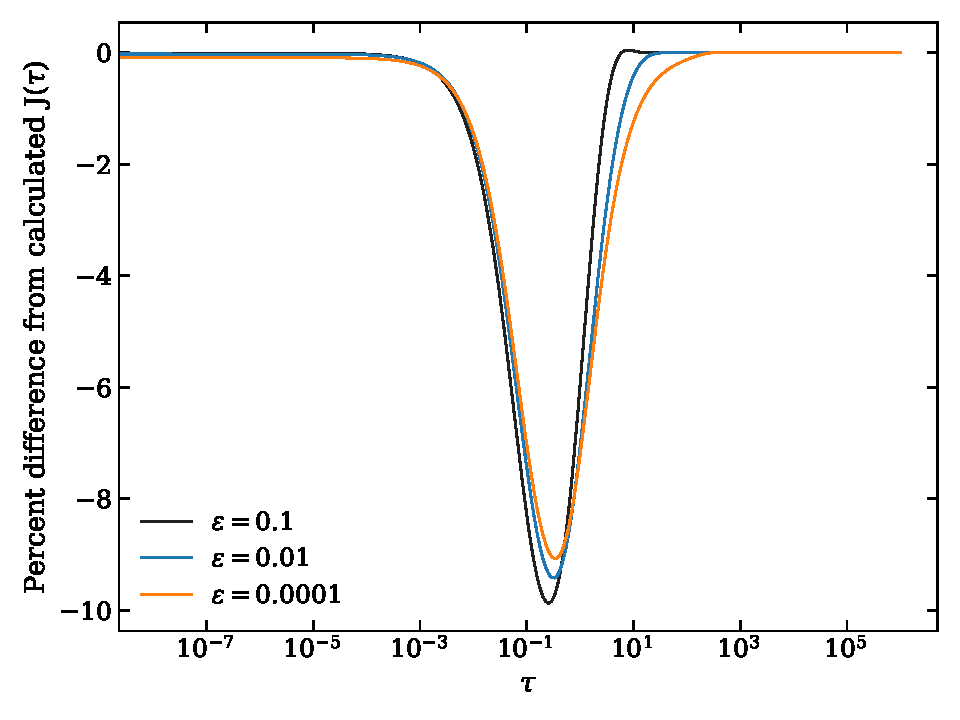
\includegraphics[width=0.75\textwidth]{J_comparison.pdf}
 \caption{Compare Eddie's J and ours (needs work)}
\end{figure}

\begin{figure}[ht]
 \centering
 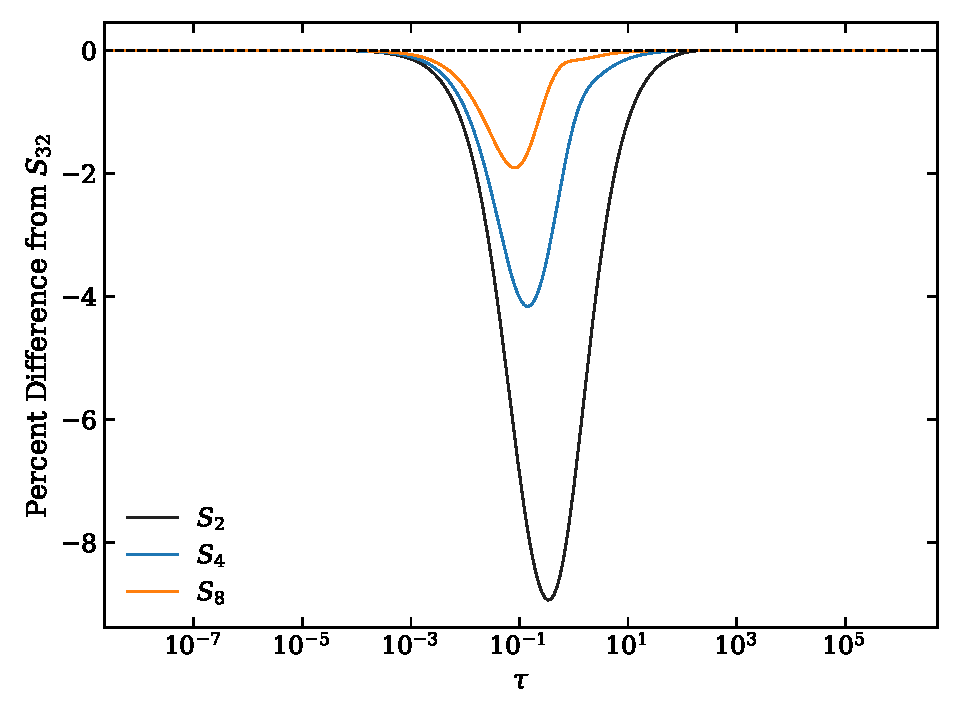
\includegraphics[width=0.75\textwidth]{quadrature.pdf}
 \caption{Deviations from 32-point Gaussian quadrature as a function of $\tau$. The greatest differences occur from 0.1 $< \tau <$ 1, where we would expect the greatest impact in the emergent flux from the atmosphere.}
\end{figure}

\begin{figure}[ht]
 \centering
 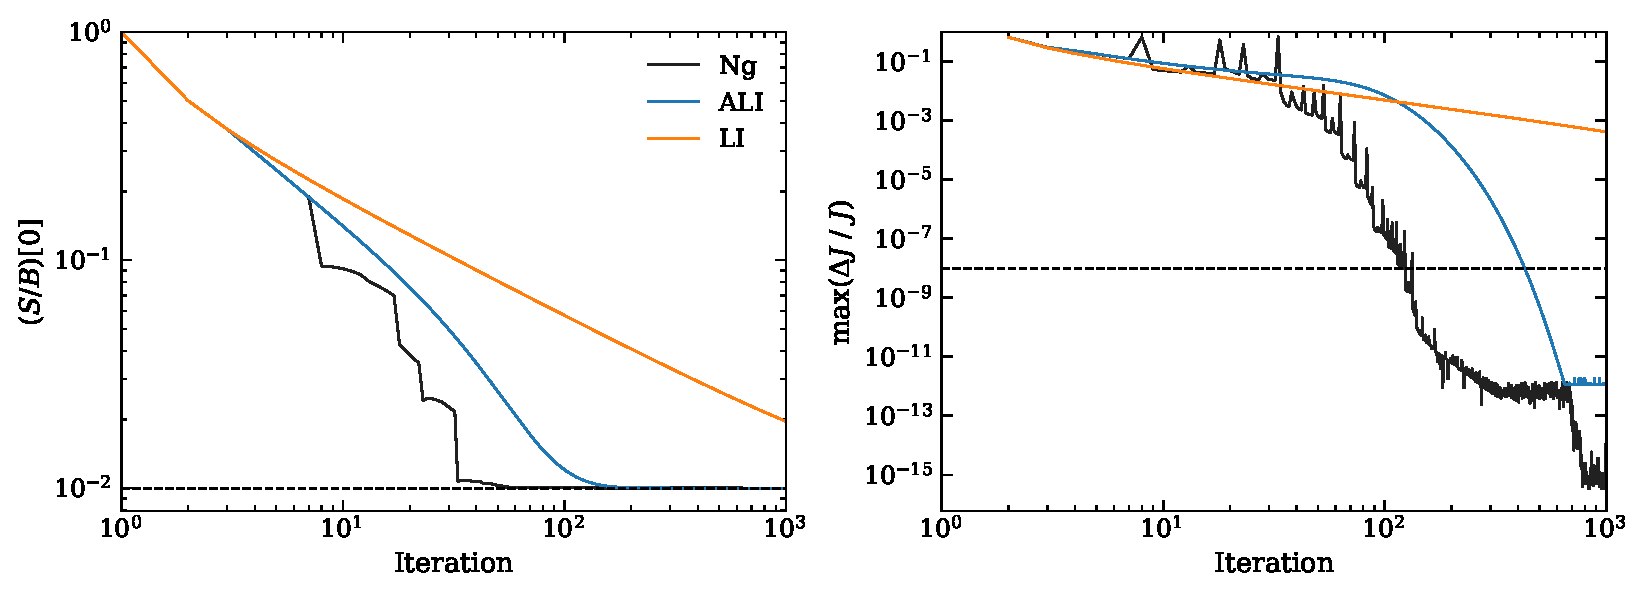
\includegraphics[width=0.75\textwidth]{iterations.pdf}
 \caption{The amount of iterations required for S/B to converge at the surface for each method used in our code. Lambda iteration takes significantly longer than ALI as expected. Ng acceleration should be even faster than ALI, but our current version does not produce that result.}
\end{figure}



-different plots
-quadrature

\section{Conclusion}



\bibliography{FinalProjectReport}

\end{document}
